\documentclass[12pt]{article}

\usepackage[left=25mm,top=12mm,bottom=20mm,right=25mm]{geometry}

\usepackage{graphicx}
\graphicspath{ {Pictures/} }

\begin{document}
\title{Project Documentation}
\author{SoftwareCide-Squad}
\maketitle

\section{Requirements}
\begin{enumerate}
\item Get data from HTML pages
\item Display it in the form of pages on the screen
\item Display some or all attributes of gathered data, depending on user preference
\item Ability to drag pages across the screen
\item Option to group sets of pages together
\item Option to remove unwanted pages from the screen
\item Option to save to other file types (e.g. excel spreadsheet)
\end{enumerate}

\section{Specifications}
\begin{enumerate}
\item Program shall get specific types of HTML pages (ebay searches, Course participants, Tutees, Module Catalog).
\item Program shall read specific data from said pages.
\item Program shall display the data in the form of one page per entry within a window.
\item Pages shall be draggable across the screen, as a real person would move real pieces of paper on a real desk.
\item Program shall allow the user to toggle whether each attribute of the entries is hidden or shown on the screen.
\item Program shall allow the user to group pages together such that they can all be moved at once.
\item Program shall allow the user to discard chosen pages.
\item Program shall allow users to export those entries which are still being displayed to other file formats, such as excel spreadsheets.
\item Program shall not allow the user to edit the data.
\end{enumerate}

\section{Sequence Diagram}
\subsection{Web scrapers}
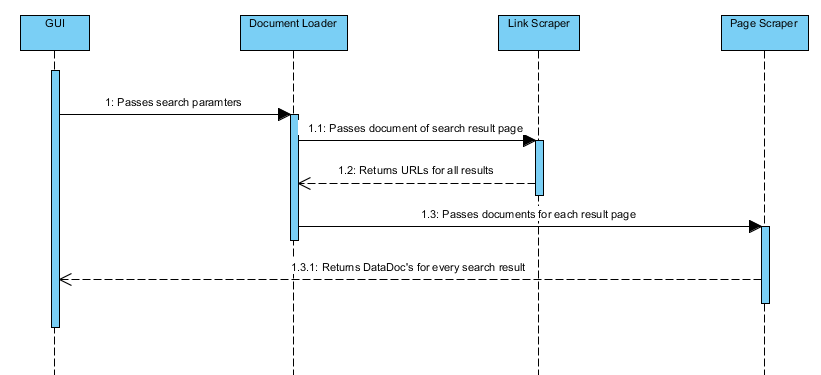
\includegraphics[scale=0.75]{ScrpSecDiag.PNG}




\end{document}
